\documentclass[UTF8]{article}

\usepackage{amsmath, amsfonts, amssymb, amstext, amscd, amsthm, bbm, CJKutf8, color, dsfont, enumerate, float, graphicx, hyperref, makeidx, mathrsfs, mathtools, marvosym, soul, url, verbatim, xcolor, xfrac}
\usepackage[left=2cm,top=2cm,right=2cm,bottom=2cm,bindingoffset=0cm]{geometry}
\allowdisplaybreaks

\newenvironment{subproof}[1][Proof]
    {\proof[#1]\leftskip=1cm\rightskip=1cm}
	{\endproof}

%theorems with custom numbering
%\newtheorem{innerthm}{Theorem}
%\newenvironment{thm}[1]
    %{\renewcommand\theinnerthm{#1}\innercustomthm}
    %{\endinnerthm}

\newtheorem{theorem}{Theorem}
\newtheorem{lemma}{Lemma}
\newtheorem{proposition}{Proposition}
\newtheorem{corollary}{Corollary}
\newtheorem{claim}{Claim}
\newtheorem{conjecture}{Conjecture}
\newtheorem{justification}{Justification}
\newtheorem{definition}{Definition}
\newtheorem*{remark}{Remark}
\newtheorem*{note}{Note}

\renewcommand{\and}{\;\wedge\;}
\newcommand{\disj}{\;\vee\;}
\newcommand{\xor}{\;\oplus\;}
\newcommand{\divides}{\;|\;}
\newcommand{\suchthat}{\;\middle|\;}
\newcommand{\contradiction}{\;\text{\Large \Lightning}}
\newcommand{\conj}[1]{\overline{#1}}
\newcommand{\mean}[1]{\overline{#1}}
\newcommand{\integral}[1]{\smashoperator{\int_{#1}}}
\renewcommand{\restriction}[1]{\downharpoonright_{#1}}
\renewcommand{\qedsymbol}{QED}

\DeclareMathOperator{\lcm}{lcm}
\DeclareMathOperator*{\argmin}{arg\!\min}
\DeclareMathOperator*{\argmax}{arg\!\max}

\let\originalleft\left
\let\originalright\right
\renewcommand{\left}{\mathopen{}\mathclose\bgroup\originalleft}
\renewcommand{\right}{\aftergroup\egroup\originalright}
\newcommand{\zh}[1]{\begin{CJK}{UTF8}{gbsn}#1\end{CJK}}
\newcommand{\jp}[1]{\begin{CJK}{UTF8}{gbsn}#1\end{CJK}}

\DeclarePairedDelimiterX \inner[2]{\langle}{\rangle}{#1,#2}
\DeclarePairedDelimiterX \braket[2]{\langle}{\rangle}{#1 \delimsize\vert #2}
\DeclarePairedDelimiter \bra{\langle}{\rvert}
\DeclarePairedDelimiter \ket{\lvert}{\rangle}
\DeclarePairedDelimiter \abs{\lvert}{\rvert}
\DeclarePairedDelimiter \lrangle{\langle}{\rangle}
\DeclarePairedDelimiter \norm{\lVert}{\rVert}
\DeclarePairedDelimiter \set{\lbrace}{\rbrace}
\DeclarePairedDelimiter \parens{(}{)}

\begin{document}
\begin{center}
	\textsc{\huge Applied Machine Learning}\\
	\textsc{\Large Homework 3}\\
\end{center}
\begin{flushright}
	Daniel Gonzalez\\
    Colton Piper\\
	$19^{\text{th}}$ of September, $2018$
\end{flushright}


\section{Results}

\subsection{Table}
We would first like to apologize for the lateness of our submission.
We initially implemented the gradient descent using bare Python list comprehensions and for-loop iteration, which turned out to be unacceptably slow.
We spent an inordinate amount of time trying to refactor that code before discovering NumPy,
after which we completely rewrote our code to take advantage of NumPy's array/vector parallelization.

Now that we were able to quickly produce data,
we tried a few different learning rates (starting with $\eta = 0.1$) before settling on a learning rate of $\eta = 1$,
which produced convergent behaviour for the \texttt{Hill-Valley} data set in around $5000$ iterations and in the \texttt{Gisette} data set in $500$ iterations.
With this learning rate, we observed convergence on the \texttt{Madelon} data set in around $4000$ iterations.
In the table below, we've compiled training and validation errors for classifiers trained on using varying numbers of iterations
(some of the lower iteration values are hold-overs from when the code ran more inefficiently).

Note the increase in the test error for \texttt{Madelon} with $10000$ iterations compared to $500$ iterations despite the decrease in training error.
This may be indicative of overfitting and could indicate that a classifier should be trained on less iterations than $10000$ for this data set.

\begin{table}[H]
\centering
    \caption{Test Misclassification Errors}
    \begin{tabular}{|c|c|c|c|}
        \hline
        \texttt{\# Data Set} & \multicolumn{1}{|c|}{\texttt{\# Iterations}} & \multicolumn{1}{|c|}{\texttt{Training Error}} & \texttt{Test Error}\\\hline
        \texttt{hill-valley} & $300$ & $48.84\%$ & $49.83\%$ \\\cline{2-4}
         & $10000$ & $46.86\%$ & $47.03\%$ \\\hline\cline{1-4}

        \texttt{madelon} & $500$ & $34.80\%$ & $41.50\%$ \\\cline{2-4}
         & $10000$ & $31.2\%$ & $42.33\%$ \\\hline\cline{1-4}

        \texttt{gisette} & $3$ & $11.87\%$ & $11.00\%$ \\\cline{2-4}
         & $15$ & $11.85\%$ & $10.90\%$ \\\cline{2-4}
         & $20$ & $11.83\%$ & $10.90\%$ \\\cline{2-4}
         & $1000$ & $5.28\%$ & $5.6\%$ \\\hline
    \end{tabular}
\end{table}

\subsection{Figures}
\begin{figure}[H]
    \centering
    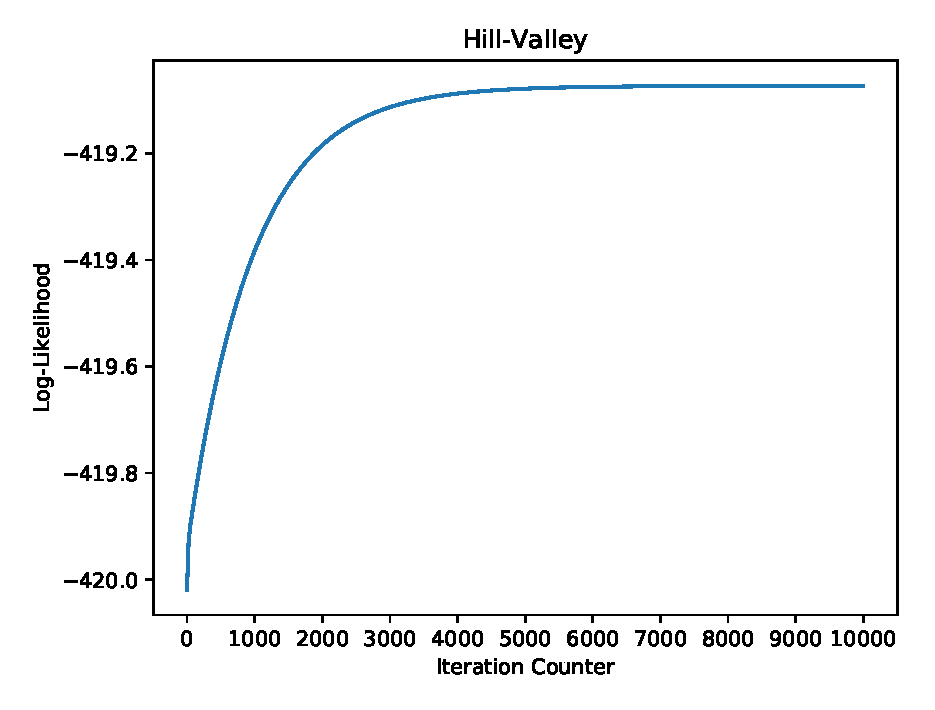
\includegraphics[scale=0.90]{./figures/hill-valley_10000_1.eps}
\end{figure}

\begin{figure}[H]
    \centering
    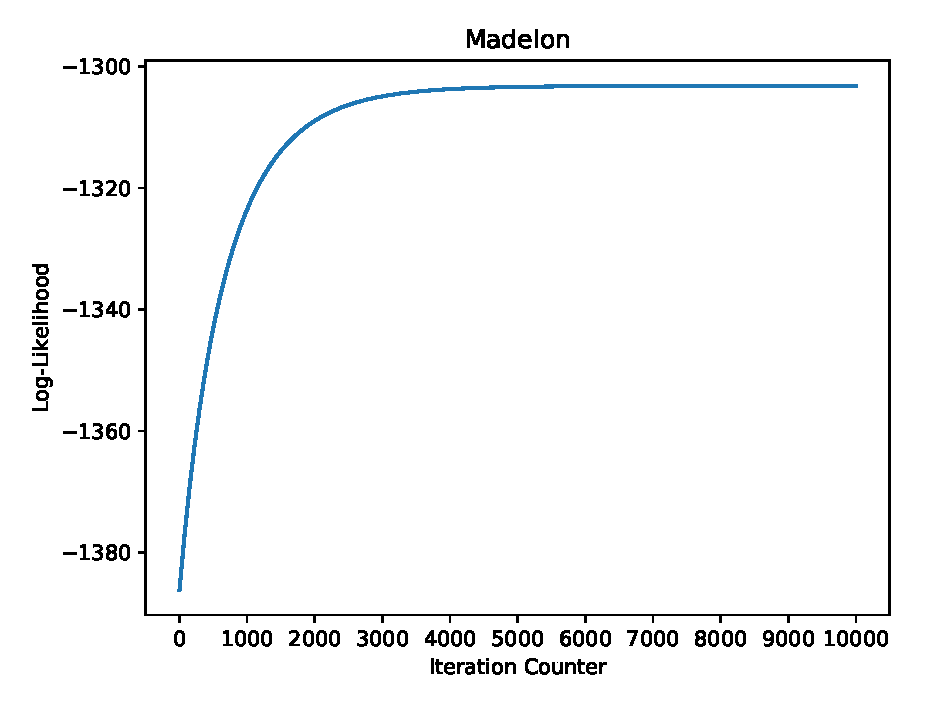
\includegraphics[scale=0.90]{./figures/madelon_10000_1.eps}
\end{figure}

\begin{figure}[H]
    \centering
    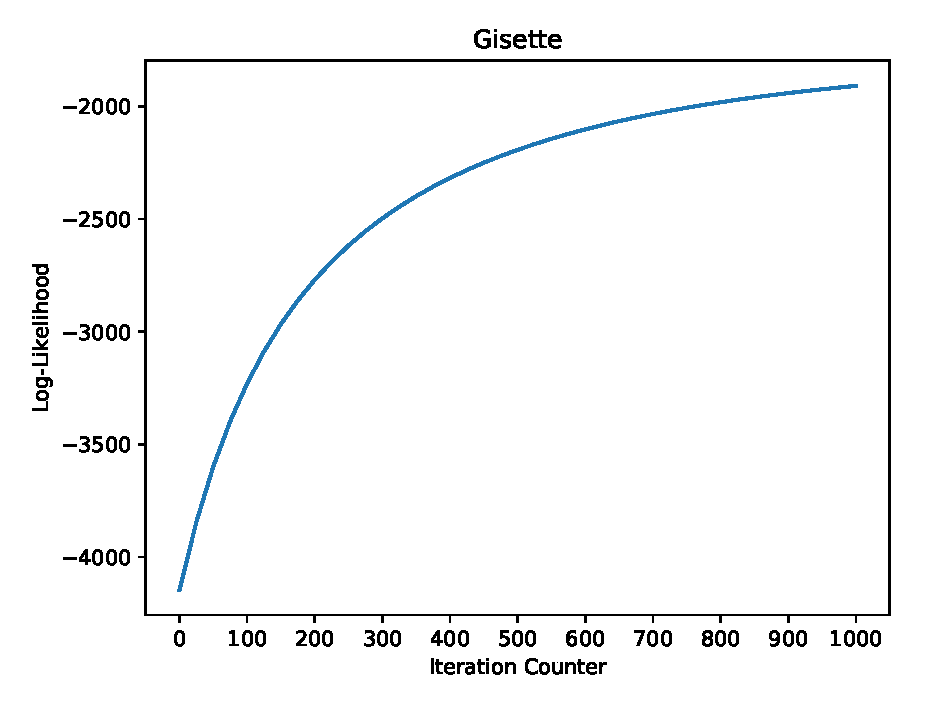
\includegraphics[scale=0.90]{./figures/gisette_500_1.eps}
\end{figure}

%\begin{figure}[H]
    %\centering
    %\includegraphics[scale=0.90]{./figures/madelon_500.eps}
%\end{figure}

%\begin{figure}[H]
    %\centering
    %\begin{minipage}{.5\textwidth}
        %\centering
        %\includegraphics[scale=0.5]{./figures/gisette_15.eps}
    %\end{minipage}%
    %\begin{minipage}{.5\textwidth}
        %\centering
        %\includegraphics[scale=0.5]{./figures/gisette_20.eps}
    %\end{minipage}
%\end{figure}

\section{Appendix: Code}
\begin{figure}[H]
    \centering
    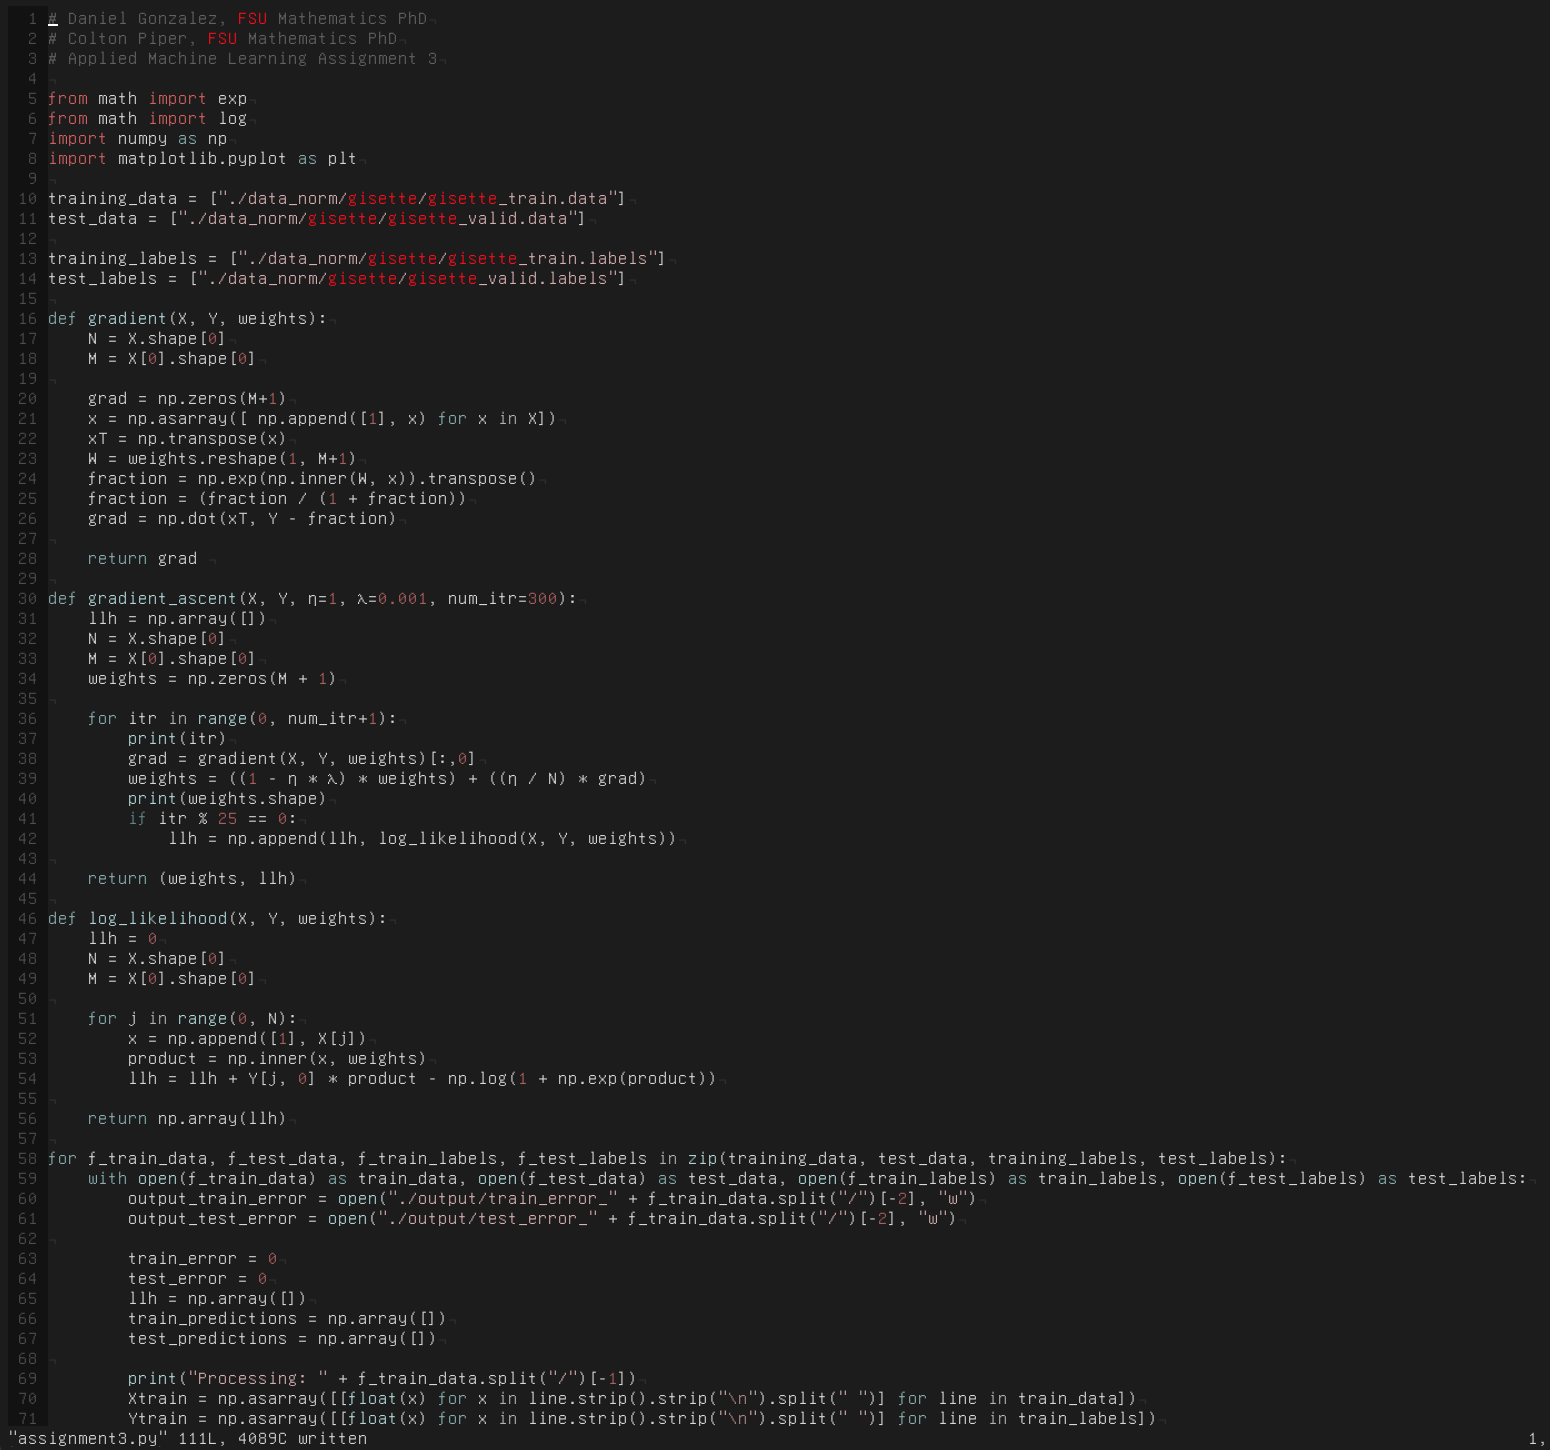
\includegraphics[scale=0.65]{./figures/code1.png}
\end{figure}
\begin{figure}[H]
    \centering
    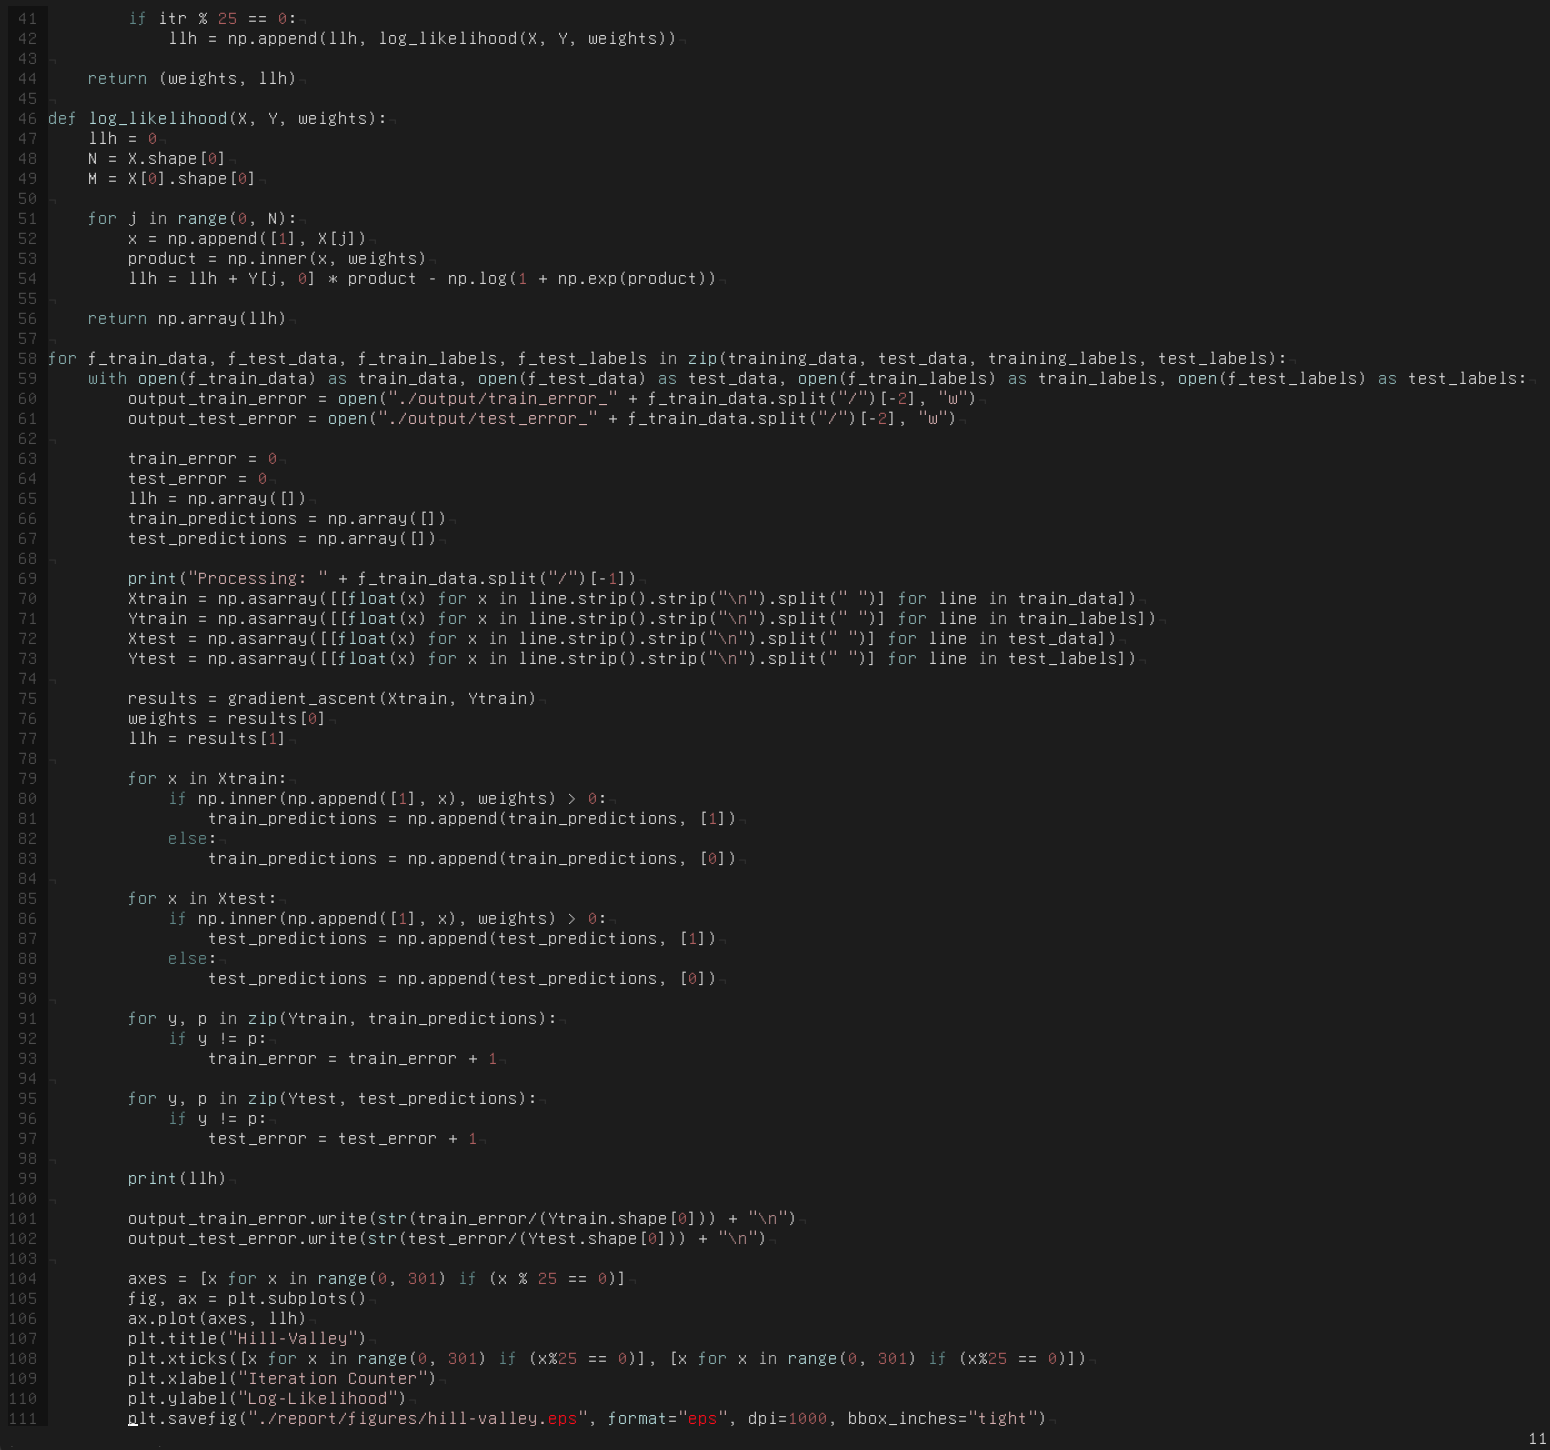
\includegraphics[scale=0.65]{./figures/code2.png}
\end{figure}

\end{document}
